\chapter{Meditation and the Sacred Mind}

This chapter follows the final movement of the San Diego dialogue on meditation. The material is not a blackboard derivation, and no validated board images remain for this lecture, but the conversation has a precise conceptual architecture. We will treat that architecture with mathematical care: not by inventing a theory, but by keeping track of implications, domains, exclusions, and transitions. The central question is whether meditation belongs to practice, control, and achievement, or whether it begins only when that whole movement is understood and ends.

\section{Control, Direction, Will, Time}

Anderson opens by recalling the previous conversation: meditation, understanding, knowledge, and the image of a flowering plant. Krishnamurti accepts the continuation and immediately returns to control. The first move is compact and severe: if the controller is not separate from the controlled, then control is not a neutral operation by an independent agent. It is one fragment attempting to dominate other fragments.

We can record the spoken sequence as a conceptual chain. This is not a formal theorem, but it is the structural spine of the opening:

\begin{equation}
\text{control}
\;\longrightarrow\;
\text{direction}
\;\longrightarrow\;
\text{will}
\;\longrightarrow\;
\text{decision or achievement}
\;\longrightarrow\;
\text{time}.
\end{equation}

The equality behind it is equally important:

\begin{equation}
\text{controller} = \text{controlled}.
\end{equation}

This identity should not be read as a psychological formula. It is Krishnamurti's way of denying a false separation. The controller is another fragment within the same field; therefore the attempt to dominate the field from outside is already confused. Once control is seen this way, direction ceases to be innocent. Direction means a projected end. The projected end implies will. Will makes a decision. Carrying out that decision requires duration. Thus control imports time into meditation.

\begin{proposition}
In the inward field described in this dialogue, psychological control contains time.
\end{proposition}

\begin{proof}
The argument is a bookkeeping argument over the lecture's own terms.
\begin{enumerate}
\item Control presupposes a controller directing what is controlled.
\item But the controller is not separate from the controlled; it is one fragment among fragments.
\item Direction establishes an end to be reached.
\item Reaching that end requires will, decision, and continuity.
\item Continuity from decision to achievement is duration.
\item Therefore psychological control contains time.
\end{enumerate}
\end{proof}

The point is not that all direction is false. That would come too quickly and would flatten the next movement of the dialogue. The point is narrower: if meditation is approached through control, then meditation has already been placed inside will, goal, and time.

\begin{figure}
\centering
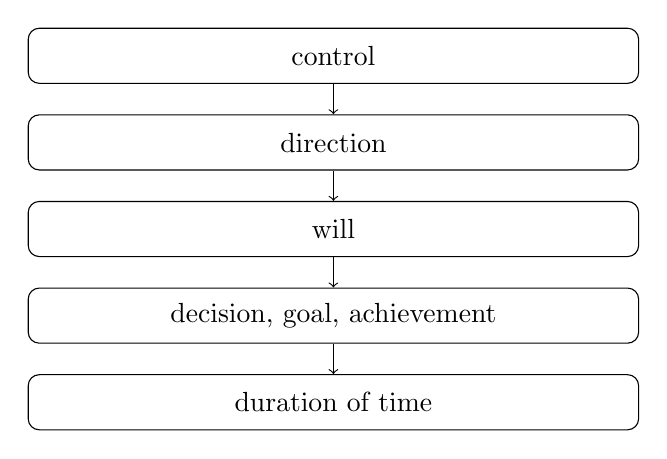
\begin{tikzpicture}
\node[draw, rounded corners, text width=0.62\linewidth, align=center, minimum height=0.7cm] (a) at (0,0) {control};
\node[draw, rounded corners, text width=0.62\linewidth, align=center, minimum height=0.7cm] (b) at (0,-1.1) {direction};
\node[draw, rounded corners, text width=0.62\linewidth, align=center, minimum height=0.7cm] (c) at (0,-2.2) {will};
\node[draw, rounded corners, text width=0.62\linewidth, align=center, minimum height=0.7cm] (d) at (0,-3.3) {decision, goal, achievement};
\node[draw, rounded corners, text width=0.62\linewidth, align=center, minimum height=0.7cm] (e) at (0,-4.4) {duration of time};
\draw[->] (a) -- (b);
\draw[->] (b) -- (c);
\draw[->] (c) -- (d);
\draw[->] (d) -- (e);
\end{tikzpicture}
\caption{A transcript-based reconstruction of the opening chain. It is not a blackboard diagram; it is a compact map of Krishnamurti's spoken sequence.}
\end{figure}

\subsection{Question \& Answer}

\paragraph{Question.}
If control implies direction, will, decision, achievement, and time, can life be lived without control, without will, and without direction?

\paragraph{Answer.}
Krishnamurti does not answer by rejecting practical intelligence. He immediately preserves a domain in which direction, calculation, decision, and choice are necessary. We need direction to go home, drive a car, speak a language, and do technical work. But in the inward field, where meditation is being discussed, choice appears because there is confusion. Where there is perception, there is no choice.

The distinction can be recorded as follows:

\begin{equation}
\text{choice without perception}
\;\longrightarrow\;
\text{confusion}.
\end{equation}

And its positive counterpart is the lecture's recurring compressed form:

\begin{equation}
\text{perception}
\;\longrightarrow\;
\text{action}.
\end{equation}

More strongly, the dialogue will later say that perception is action. There is no interval between seeing danger and acting. For the present stage, the key is that meditation is not one more controlled activity. If it is controlled, it remains inside will and time.

\section{The Field of Knowledge and the Inward Field}

Anderson then presses a necessary clarification. Will seems to have a valid place in ordinary knowledge. Decision belongs to know-how. Choice belongs to technical and practical life. Krishnamurti agrees. The mistake is not practical decision; the mistake is carrying the movement of practical decision into inward order.

\begin{table}
\centering
\begin{tabular}{p{0.43\linewidth} p{0.43\linewidth}}
\textbf{Field of knowledge} & \textbf{Inward field} \\
Direction, calculation, decision, and choice are necessary. & Psychological direction, will, and choice indicate confusion. \\
Driving, language, technology, and ordinary navigation belong here. & Meditation, perception, attention, and inward order belong here. \\
Choice compares this with that. & Perception sees directly; action is not delayed by choice. \\
\end{tabular}
\caption{A narrow working distinction. The point is not anti-intellectualism; it is the non-transferability of the practical pattern into inward order.}
\end{table}

The danger of confusing the two fields is sharper than it first appears. We may think that one can be efficient in knowledge and inwardly disordered, as though these were two separate compartments. Krishnamurti rejects that division. As long as one is not completely in order inwardly, even outward action is touched by disorder. Anderson identifies the same problem as the false split between inner and outer; Krishnamurti attributes that split to thought.

So the draft should not say merely: knowledge is outer, meditation is inner. The lecture is subtler. Thought has divided the outer and the inner, and that very division is part of the disorder. The valid distinction is not a metaphysical wall; it is a functional distinction between necessary practical knowledge and the confusion caused by importing will into meditation.

\section{From Direction to Space}

Once direction has been linked with time, Krishnamurti pivots to space. He does not begin with inward space. He first moves through ordinary space: mountains, trees, flowers, crowded apartments, cities spreading, people breathing the same air, thinking the same thoughts, carrying the same anxieties and fears. Space is necessary; without it there is stifling.

The inward turn comes after this concrete setup. Can the mind have space? Krishnamurti answers by returning to the earlier chain:

\begin{equation}
\text{direction}
\;\longrightarrow\;
\text{time}
\;\longrightarrow\;
\text{no inward space}.
\end{equation}

Occupation is another way of saying the same thing. A mind filled with family, business, God, drink, sex, experience, knowledge, and thought has no space. The words are deliberately ordinary. The point is not that these matters never arise. It is that occupation fills the whole field.

\begin{equation}
\text{occupation by thought and knowledge}
\;\longrightarrow\;
\text{no space}.
\end{equation}

Thought also creates a small enclosure around itself: me and you, we and they. The self lives in that little space. To move out of it is felt as terror, fear, and anxiety, because that enclosure is the familiar field of being. Meditation is therefore described as the freeing of the mind from its content as consciousness.

\begin{definition}
In this dialogue, inward space is not a private possession of the self. It is the ending of the little space created by thought as ``me'' and ``mine.''
\end{definition}

This is why outward space cannot give inward space. One may go to the country or take a vacation, but without understanding the movement of occupation one merely goes from one enclosure to another. The inward space in question begins when occupation ends; when what has to be done is done, the mind does not carry it onward as psychological residue.

\section{Space Means Silence}

The next pivot is terse: space means silence. Again, the lecture proceeds by exclusion. Silence is not the space between two noises. It is not the cessation of noise. It is not something thought has produced. It is not the result of practice. It is not the atmosphere of a church or temple. These exclusions matter because they prevent the word from becoming sentimental or decorative.

We can preserve the logic by writing the negative definition as a set of exclusions:

\begin{align}
\text{silence} \neq{}&
\text{interval between noises}, \\
\text{silence} \neq{}&
\text{mere cessation of noise}, \\
\text{silence} \neq{}&
\text{a state produced by thought}, \\
\text{silence} \neq{}&
\text{a result induced by practice}.
\end{align}

This is not a mathematical definition in the strict sense. It is a guardrail. The lecture refuses to let silence become either an acoustic condition or an achievement.

\subsection{Question \& Answer}

\paragraph{Question.}
Can this silence operate in daily life, while we still live in the field of knowledge?

\paragraph{Answer.}
Krishnamurti says it can. The answer is not withdrawal from knowledge. We still live in knowledge; we still speak, work, calculate, and act practically. The question is whether silence and knowledge can move together without division. The image is of two rivers flowing in balance.

The note form is:

\begin{equation}
\text{knowledge in practical life}
\;+\;
\text{silence without division}
\;\longrightarrow\;
\text{harmony}.
\end{equation}

If this is not possible, then one can only live in the field of knowledge. But for Krishnamurti the possibility is real. He does not present it as a method to be reached by vanity or attainment; he states it as a fact of living. This answer opens the next question: if silence can operate in daily life, what is creation?

\section{Creation, Measure, and the Immeasurable}

Creation is introduced only after control, knowledge, space, and silence have been worked through. This order is essential. If creation is discussed too early, it becomes expression: painting, writing, composing, making a statue, producing a child, pressing something out of oneself. Anderson notes the literal sense of expression as something pressed out; Krishnamurti accepts that danger. A writer may be in conflict, in tension, and out of that conflict produce a book. That may be expression, but it is not what is meant here by creation.

Creation is described as flowering in which the flower does not know that it is flowering. The chapter should retain the image, because it links back to the opening and forward to the ending of suffering.

The sharper conceptual move follows:

\begin{equation}
\text{thought} = \text{measure}.
\end{equation}

As long as thought is cultivated as the basis of action, the search for the immeasurable has no meaning. One may assert the eternal, the unnameable, or the sacred, but such assertion remains supposition or speculation. The movement of thought cannot produce the immeasurable, because it remains within measure.

\begin{proposition}
Within the terms of the dialogue, the immeasurable is not reached by a measured movement of thought.
\end{proposition}

\begin{proof}
\begin{enumerate}
\item Thought is named as measure.
\item A search conducted by thought is therefore a movement within measure.
\item The immeasurable cannot be the product of the measured.
\item Therefore the search for the immeasurable through thought has no meaning.
\end{enumerate}
\end{proof}

This is one of the chapter's cleanest logical turns. The statement is not that the immeasurable is denied. Rather, the route of speculation, assertion, and thought-made religion is denied.

\section{Energy, the Sacred, and Secondary Powers}

When the mind is utterly silent, the dialogue says, not a thing is wasted. There is no dissipation of energy. The word energy should be kept close to the transcript. It is not a physics term here. It names the gathered force of a mind without conflict, control, reaching, seeking, asking, waiting, or praying.

A useful compact form is:

\begin{equation}
\text{silence}
-
\{\text{conflict},\text{control},\text{seeking},\text{asking},\text{praying}\}
\;\longrightarrow\;
\text{gathered energy}.
\end{equation}

And the later formulation is:

\begin{equation}
\text{attention}
\;\approx\;
\text{gathering of all energy}.
\end{equation}

The approximation sign is intentional. It marks an editorial shorthand, not a literal equivalence. Krishnamurti says religion is the gathering of all energy, which is attention. The notes can preserve this relation while avoiding a false technical model.

\begin{figure}
\centering
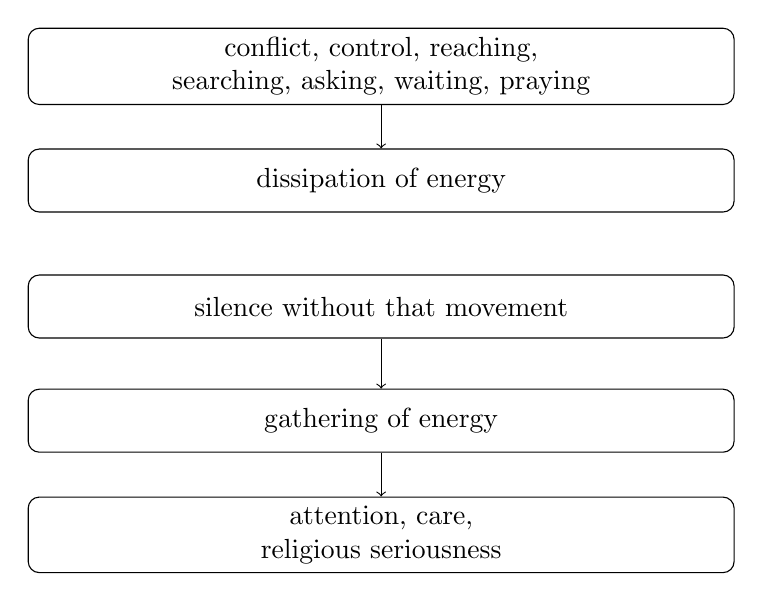
\begin{tikzpicture}
\node[draw, rounded corners, text width=0.72\linewidth, align=center, minimum height=0.8cm] (a) at (0,0) {conflict, control, reaching,\\ searching, asking, waiting, praying};
\node[draw, rounded corners, text width=0.72\linewidth, align=center, minimum height=0.8cm] (b) at (0,-1.45) {dissipation of energy};
\node[draw, rounded corners, text width=0.72\linewidth, align=center, minimum height=0.8cm] (c) at (0,-3.05) {silence without that movement};
\node[draw, rounded corners, text width=0.72\linewidth, align=center, minimum height=0.8cm] (d) at (0,-4.5) {gathering of energy};
\node[draw, rounded corners, text width=0.72\linewidth, align=center, minimum height=0.8cm] (e) at (0,-5.95) {attention, care,\\ religious seriousness};
\draw[->] (a) -- (b);
\draw[->] (c) -- (d);
\draw[->] (d) -- (e);
\end{tikzpicture}
\caption{A transcript-based reconstruction of the energy movement. The diagram avoids treating energy as a physical variable.}
\end{figure}

The silence in which energy is gathered is called sacred. But the lecture immediately distinguishes this from the sacred thing invented by thought. A sacred image, word, doctrine, or projection is not the sacred mind being described. When the mind itself becomes sacred, Krishnamurti says, it opens the door to something immeasurably sacred. Religion, in this use, is not belief but a quality of living that affects speech, conduct, relationship, and care.

The dialogue then checks a temptation. When energy is gathered, powers may appear: healing, miracles, extrasensory capacities. Krishnamurti does not deny that such things may occur; he says they are secondary and dangerous. The danger is simple:

\begin{equation}
\text{talent or power}
\;\longrightarrow\;
\text{importance of me}
\;\longrightarrow\;
\text{position, money, worship}.
\end{equation}

The religious mind, in the sense used here, does not build identity on these powers. It puts them away. This is not indifference to people; it is the refusal to let secondary issues revive the self.

\section{Prayer, Books, Attention, and the Ending of Suffering}

The last major test is prayer. Anderson asks about prayer in relation to meditation, since convention often joins the two. Krishnamurti answers directly: prayer as petition has no place in meditation. To whom is one praying? Whom is one asking? Petition belongs to conflict, sorrow, lack, fear, and the desire to achieve.

\subsection{Question \& Answer}

\paragraph{Question.}
If prayer is not petition, is there any use of the word that belongs with meditation?

\paragraph{Answer.}
The lecture does not develop a positive doctrine of prayer. It removes petition. When there is no petition, there is no asking. When there is no asking, one can look. Anderson names this immense quietude; Krishnamurti calls it real peace. Thus the practical relation is:

\begin{equation}
\text{no petition}
\;\longrightarrow\;
\text{no asking}
\;\longrightarrow\;
\text{looking}
\;\longrightarrow\;
\text{real peace}.
\end{equation}

The examples are deliberately plain: praying for a refrigerator, praying for peace while living violently, praying for one's country while sustaining division. These examples keep the discussion from becoming abstract. Petition reproduces the very disorder from which it asks to be saved.

From prayer the dialogue turns to books and teachers. Books have become important; the mind becomes second-hand through what others have said about reality. Krishnamurti's question is whether such a mind can come upon what is original. The answer follows the same pattern as before: no teacher can teach this, because the teacher and the taught are not finally separate in the way we imagine. The disciple is the teacher.

The final return is to seriousness. Meditation is not an activity one does among other activities. It means attention and care: care for children, neighbor, country, earth, trees, and animals. Seriousness brings attention, care, and responsibility; one does not proceed through a program of stages but sees.

The closing chain is:

\begin{equation}
\text{perception}
\;\longrightarrow\;
\text{action}
\;\longrightarrow\;
\text{wisdom}
\;\longrightarrow\;
\text{ending of suffering}.
\end{equation}

Suffering is not ended by refusal, rationalization, escape, or the decision to go beyond it. It is observed. It flowers, and in choiceless awareness it withers away. This returns us to the opening image of the flower, now sharpened by the whole lecture. Desire, will, suffering, and creation have all been understood through flowering without coercion.

At the very end Anderson speaks of energy free to pattern itself or not to pattern itself. Krishnamurti adds the final sentence of the argument: in silence, time stops. The formula must remain cautious, but it belongs as the chapter's closing mark:

\begin{equation}
\text{silence}
\;\longrightarrow\;
\text{time stops}.
\end{equation}

\section{Summary}

The lecture proceeds by tightening one term into the next. Control reveals direction; direction reveals will; will reveals decision and time. The first decisive distinction is between the field of knowledge, where direction and choice are necessary, and the inward field, where choice indicates confusion and perception acts without interval.

From time the dialogue moves to space. Thought creates a little space around the self, and occupation fills the mind. Meditation is the freeing of the mind from that content. Space then becomes silence, but silence is protected from false definitions: it is not noise management, not practice, not thought-made quiet.

The culmination is the gathering of energy in silence. That gathered energy is attention, care, and religious seriousness. It is sacred only when it is not a sacred thing invented by thought. Powers, prayer, books, and teachers are then tested as possible diversions. The chapter ends where the whole dialogue has been moving: perception is action, wisdom is the ending of suffering, and in silence time stops.